\subsubsection{Pianosa}
On this architecture, due to the lack of space on disks, we will be able to test Sorting Algorithms for data sets of size at most 4GB, namely 1G integers. Further, given the results of tests shown in~\ref{test-env-pianosa}, the size of the communication buffer of the DAL layer has been set to 32MB. We have also practically experienced that a larger buffer, in general, does not give significant benefits, while a shorter one impair a little the Time Completion.

\paragraph{Scalability of Sorting Algorithms}
Figures~\ref{NxTxM} and~\ref{MxTxN} show the Time Completion of Sorting Algorithms on Pianosa.

If the data set is \textbf{small} (i.e. of size up to 64MB) there is not any Sorting Algorithms that shows a good scalability. Even worse, if we look at Figure~\ref{NxTxA-small} we notice that by increasing the parallelism degree we obtain an increase of the Time Completion too. In reality, this behaviour is not surprising. The cost of \textit{Sequentialsort} (that is, the cost of the standard \textit{ANSI qsort}, since the data set surely fits the primary memory) for small data sets varies between a few seconds and tens of milliseconds, that is the same order magnitude of $T\_send( \sim KB )$ (see~\ref{test-env-pianosa} for more details). This means that the cost of communications between processes has a significative impact on the final performance of Sorting Algorithms. From a qualitative point of view, the higher the parallelism degree, the higher both the number of communications and the overall time spent in sending datas, so higher is even the overhead introduced by the parallelization. This is why Sorting Algorithms cannot scale and usually exhibit a Time Completion even worse than the one of \textit{Sequentialsort}.

Things are a little bit different when the data set is \textbf{large}, namely when its size is between 128MB and 512MB. Figure~\ref{NxTxM} clearly shows that there is not any algorithm that scales. Bucketsort and Samplesort have a little improvement passing from $n=2$ to $n=4$, but nothing extraordinary. However, if the data set is of 512MB, the parallelization is useful to lower the Time Completion with respect to the one of \textit{Sequentialsort}. Figure~\ref{sequential-pianosa} shows that, for sorting 512 MB, \textit{Sequentialsort} takes roughly 400s, while all Sorting Algorithms, except Quicksort, are able to lower it up to roughly 200s with just $n=4$. Unfortunately, we do not obtain any further improve neither moving from $n=4$ to $n=8$ nor considering a smaller data size (with just $M=256MB$ the parallelizzation gain is not significative). Reasons are quite obvious. From one hand, if we increase the parallelism degree the negative impact of communications is greater than the gain coming from having more computational units (working on smaller partitions).  From the other hand, $M=512MB$ means a jump to an important computational grain: indeed, moving from $n=2$ to $n=4$ guarantees processes to work with a partition of the data set that is still significative; this explains why some Sorting Algorithms shows a gain in terms of Time Completion within this range of processes. If we further increase $n$ up to $16$, processes have to work on smaller partitions, which let the parallelization in some sense useless.

Summarizing, we have just seen that Sorting Algorithms do not scale with data sets of sizes up to a few hundreads of megabytes. Moreover, for small data sets, \textit{Sequentialsort} even outperforms all other parallel algorithms. Reasons of this behaviour are mainly two: the fine grain computation on a few datas \textit{and} the cost of communications, which becomes predominant on a cluster. Now, we focus on \textbf{huge} data sets. Even if the computation is still of fine grain, now each process works with larger partitions of the data set. Besides, notice that in our tests the increment of the data set size is exponential (doubles at each test). This means that processes spend greatly more time in computation than what happened for large data sets. Just as an example, think to two data sets $A$ and $B$, the former of size $\sharp A = 256$ MB, the latter of size $\sharp B = 2$ GB; both of them have to be sort with the same generic Sorting Algorithm. Assume that the parallelism degree is $n=8$. In the first phases of the algorithm, each process works with partitions of sizes respectively $local_A = \frac{\sharp A}{n} = 32$ MB and $local_B = \frac{\sharp B}{n} = 256$ MB. It is clear that a lot of more time is spent just to sort local partitions. If the Sorting Algorithm has a parallel logic such that both the workload keeps balanced among processes and the amount of communications do not overcome the time spent in computations, then a Sorting Algorithm \textit{can} scale. For instance, assume that the Sorting Algorithm in question is the \textit{Samplesort}. During the various steps of the algorithm, processes work with partitions of similar sizes and, except in both the initial scattering and final gathering phases, on average they send $local_{\lbrace A,B \rbrace}$ datas (see~\ref{Samplesort}). On the other hand, assume that the Sorting Algorithm is the \textit{Mergesort}. It is still true that when the data set is $B$, processes have a larger computation phase: but it is also true that the workload tends to be concentrated on a few processes through $log_2{n}$ phases of costly communications (in the best case, a process sends $local_{\lbrace A,B \rbrace}$, while in the final step of the algorithm a process has to send $\frac{\sharp\lbrace A,B\rbrace}{2}$ datas). Therefore, this example shows intuitively how for some Sorting Algorithms (in our case \textit{Samplesort}) the increase of the data set size implies a larger increment of the computation phase with respect to the communication phase, while for other algorithms (in our case \textit{Mergesort}) the workload gets unbalanced after costly phases of communications. This example was necessary to give an idea of why we obtain the behaviour shown in Figure~\ref{NxTxM}, where for huge data sets only some Sorting Algorithms significatively improve their Time Completion by increasing $n$ (\textit{Bucketsort}, \textit{Samplesort}, \textit{Load-Balanced (Multi-Way) Mergesort}, \textit{Bitonicsort}), while other either do not get better (\textit{Mergesort}, \textit{4-Way Mergesort}) or even worsen (\textit{Quicksort}). However, notice that in every case the scalability is far away from the ideality. 

Finally, we observe an interesting behaviour. We consider again the Time Completion of Sorting Algorithms in case of huge data sets. Figure~\ref{NxTxM} shows that algorithms like \textit{Samplesort} (Figure~\ref{NxTxM-samplesort}) and \textit{Load-Balanced Multi-Way Mergesort} (Figure~\ref{NxTxM-lbkmergesort}) exhibit the best gain when the parallelism degree grows from 2 to 4, while by passing to 8 and even worse to 16 the gain tends to diminish. There are no valid reasons to think that with higher parallelism degree the gain restarts to grow. On the other hand, \textit{Bitonicsort} (Figure~\ref{NxTxM-bitonicsort}) does not obtain a significative gain with parallelism degrees up to 8, while passing from 8 to 16 the gain nearly halves. Therefore, it would be interesting to study the behaviour of \textit{Bitonicsort} for higher parallelism degree; this will be our matter of study on another target architecture.


\begin{figure}[t]
    \begin{center}
        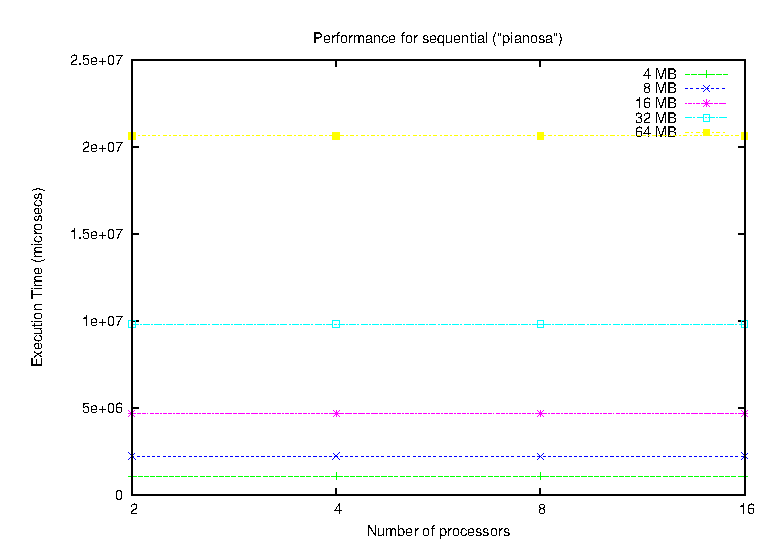
\includegraphics[scale=0.6]{plots/test_01_pianosa/NxTxM/sequential_pianosa_NxTxM_small}
    \end{center}
    
    \begin{center}
        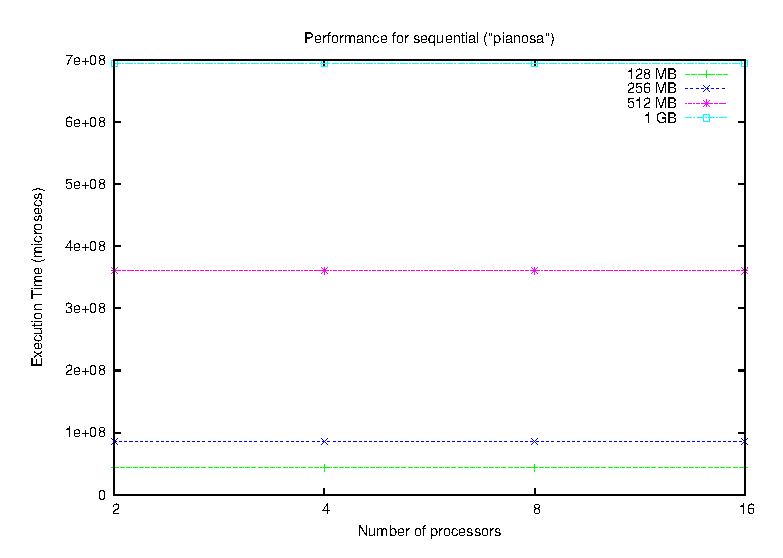
\includegraphics[scale=0.6]{plots/test_01_pianosa/NxTxM/sequential_pianosa_NxTxM_large}
    \end{center}
    
    \begin{center}
        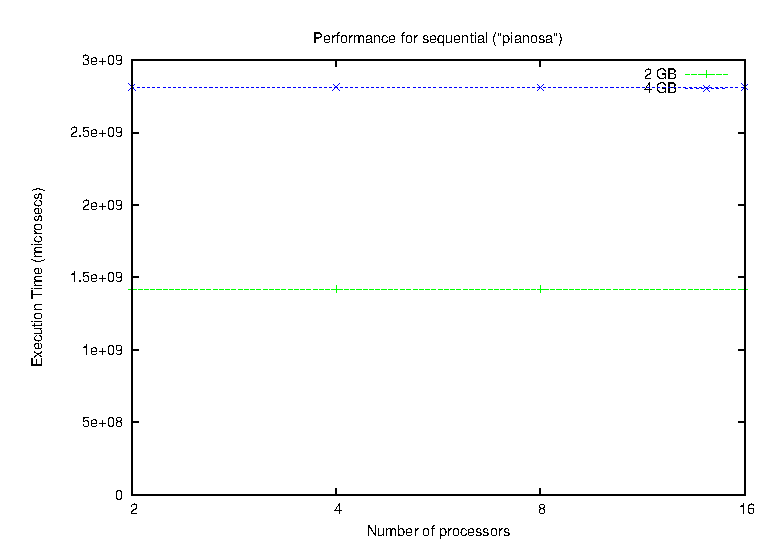
\includegraphics[scale=0.6]{plots/test_01_pianosa/NxTxM/sequential_pianosa_NxTxM_huge}
    \end{center}
    \caption{\textit{Pianosa}. Completion Time for the Sequentialsort.}
    \label{sequential-pianosa}
\end{figure}

%%%%%%%%%%%%%%%%%%%%%%%%%%%%%%%%%%%%%%%% Small data set %%%%%%%%%%%%%%%%%%%%%%%%%%%%%%%%%%%%%%%%%%%%%%%%%%%%%%
\begin{figure}[h]
    \centering
    \subfloat[Quicksort.]{\label{NxTxM_small-quicksort}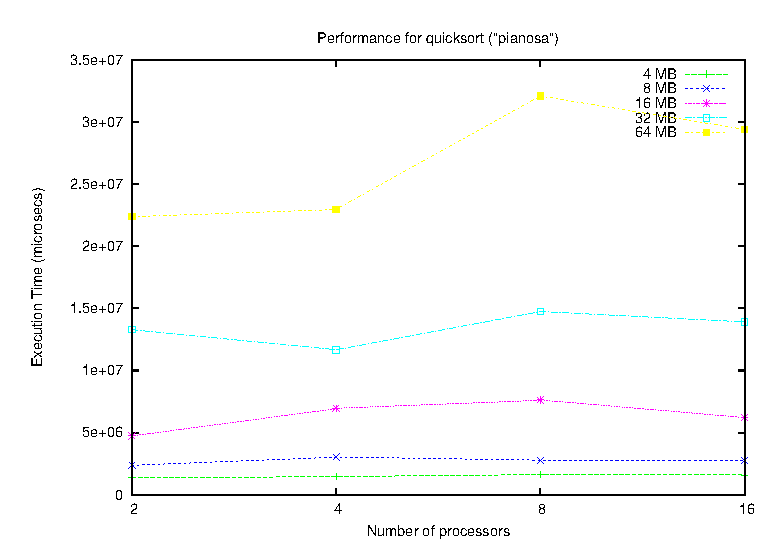
\includegraphics[width=0.4\textwidth]{plots/test_01_pianosa/NxTxM/quicksort_pianosa_NxTxM_small}} 
    \hspace*{20pt}  
    \subfloat[Bitonicsort.]{\label{NxTxM_small-bitonicsort}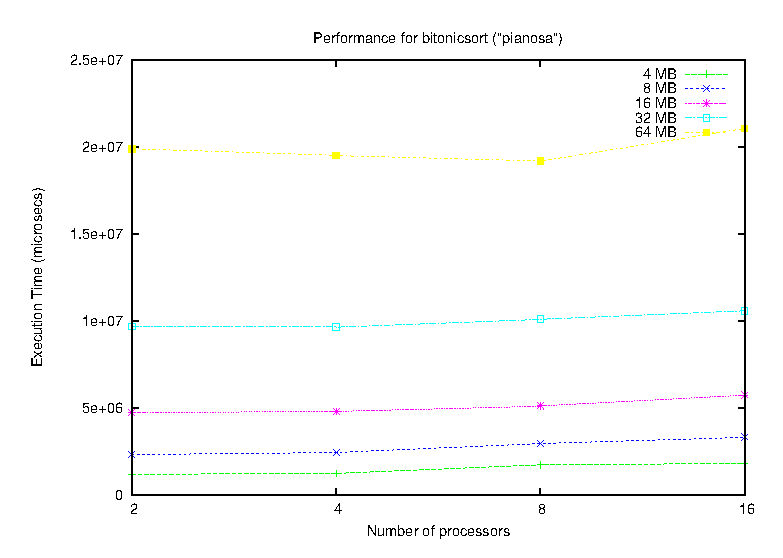
\includegraphics[width=0.4\textwidth]{plots/test_01_pianosa/NxTxM/bitonicsort_pianosa_NxTxM_small}} 
    
    \centering
    \subfloat[Bucketsort.]{\label{NxTxM_small-bucketsort}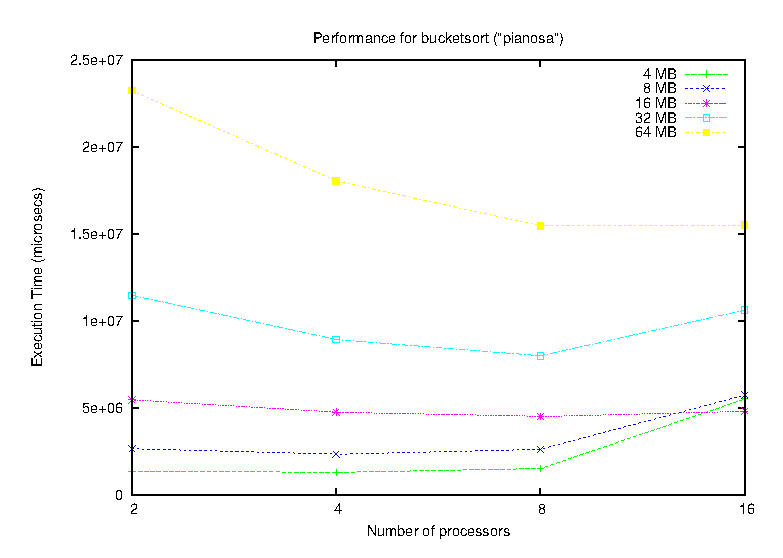
\includegraphics[width=0.4\textwidth]{plots/test_01_pianosa/NxTxM/bucketsort_pianosa_NxTxM_small}} 
    \hspace*{20pt}
    \subfloat[Samplesort.]{\label{NxTxM_small-samplesort}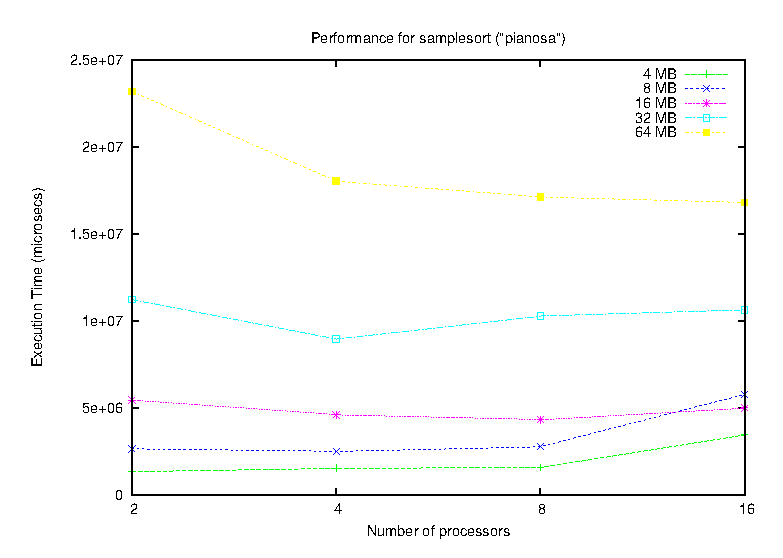
\includegraphics[width=0.4\textwidth]{plots/test_01_pianosa/NxTxM/samplesort_pianosa_NxTxM_small}} 
    
    \centering
    \subfloat[Mergesort.]{\label{NxTxM_small-mergesort}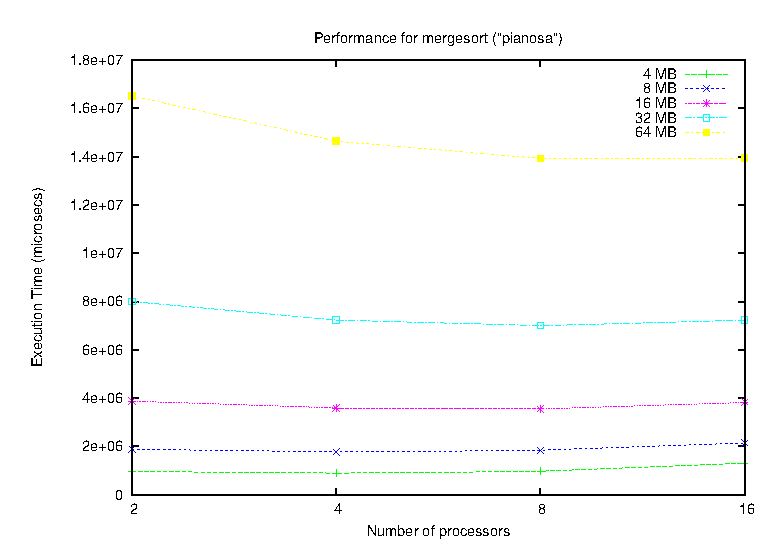
\includegraphics[width=0.4\textwidth]{plots/test_01_pianosa/NxTxM/mergesort_pianosa_NxTxM_small}}   
    \hspace*{20pt}  
    \subfloat[4-Way Mergesort.]{\label{NxTxM_small-kmerge}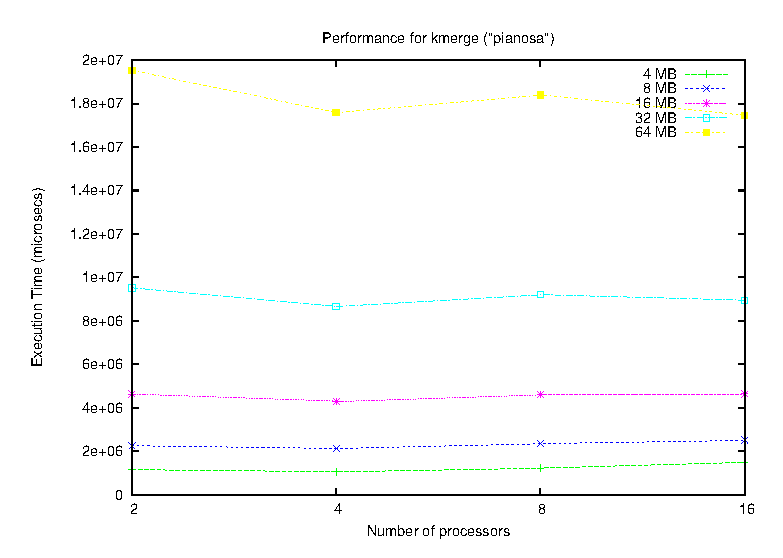
\includegraphics[width=0.4\textwidth]{plots/test_01_pianosa/NxTxM/kmerge_pianosa_NxTxM_small}} 
    
    \centering
    \subfloat[Load-Balanced Mergesort.]{\label{NxTxM_small-lbmergesort}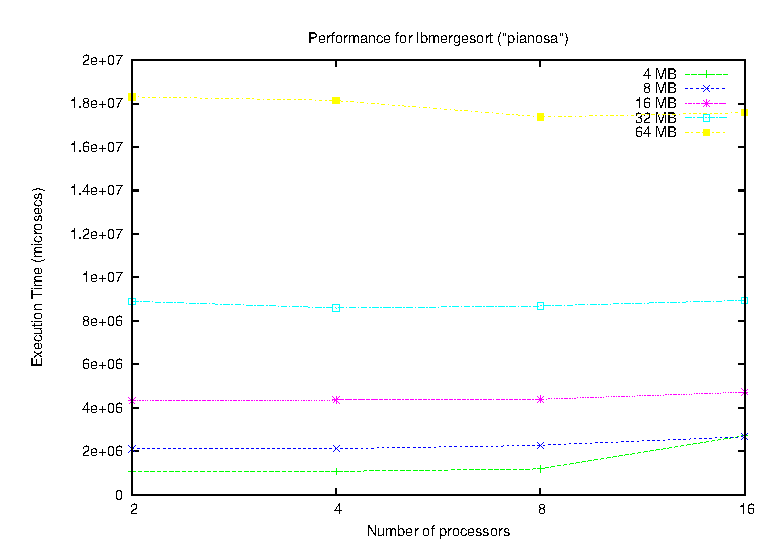
\includegraphics[width=0.4\textwidth]{plots/test_01_pianosa/NxTxM/lbmergesort_pianosa_NxTxM_small}} 
    \hspace*{20pt}  
    \subfloat[Load-Balanced Multi-Way Mergesort.]{\label{NxTxM_small-lbkmergesort}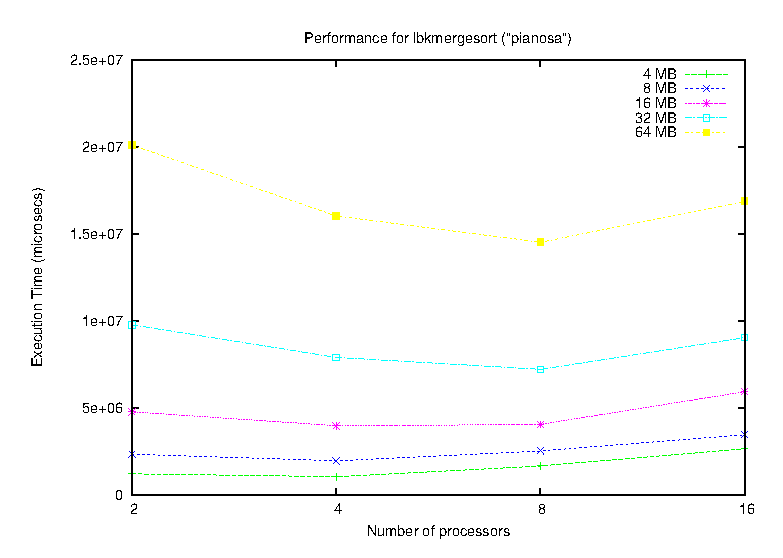
\includegraphics[width=0.4\textwidth]{plots/test_01_pianosa/NxTxM/lbkmergesort_pianosa_NxTxM_small}}  
    
\end{figure}



  
%%%%%%%%%%%%%%%%%%%%%%%%%%%%%%%%%%%%%%%% Large data set %%%%%%%%%%%%%%%%%%%%%%%%%%%%%%%%%%%%%%%%%%%%%%%%%%%%%%
\begin{figure}[h]
	\ContinuedFloat
	 
    \centering
    \subfloat[Quicksort.]{\label{NxTxM_large-quicksort}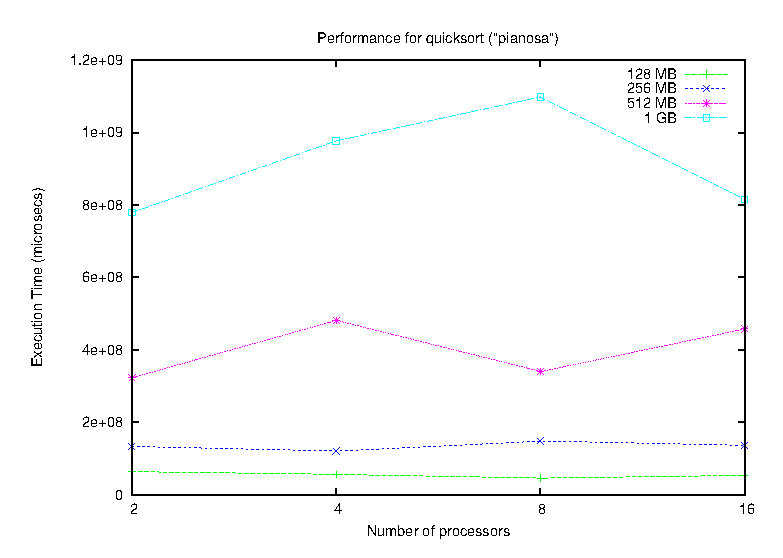
\includegraphics[width=0.4\textwidth]{plots/test_01_pianosa/NxTxM/quicksort_pianosa_NxTxM_large}} 
    \hspace*{20pt}  
    \subfloat[Bitonicsort.]{\label{NxTxM_large-bitonicsort}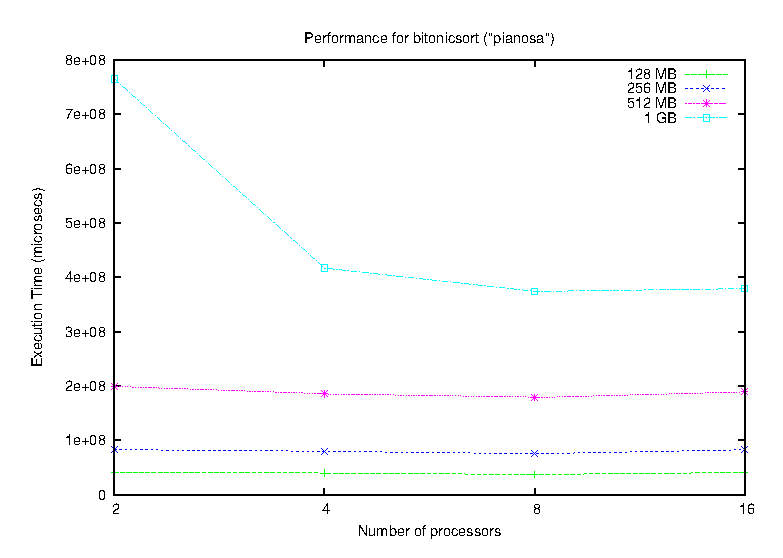
\includegraphics[width=0.4\textwidth]{plots/test_01_pianosa/NxTxM/bitonicsort_pianosa_NxTxM_large}} 
    
    \centering
    \subfloat[Bucketsort.]{\label{NxTxM_large-bucketsort}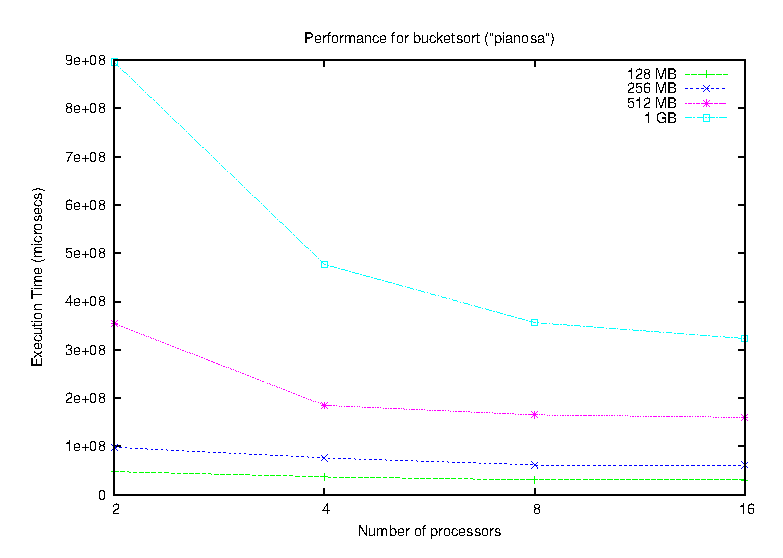
\includegraphics[width=0.4\textwidth]{plots/test_01_pianosa/NxTxM/bucketsort_pianosa_NxTxM_large}} 
    \hspace*{20pt}
    \subfloat[Samplesort.]{\label{NxTxM_large-samplesort}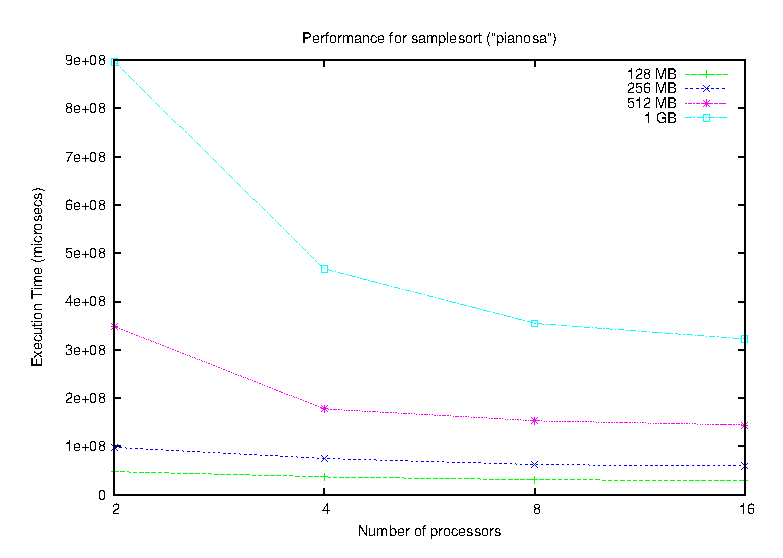
\includegraphics[width=0.4\textwidth]{plots/test_01_pianosa/NxTxM/samplesort_pianosa_NxTxM_large}} 
    
    \centering
    \subfloat[Mergesort.]{\label{NxTxM_large-mergesort}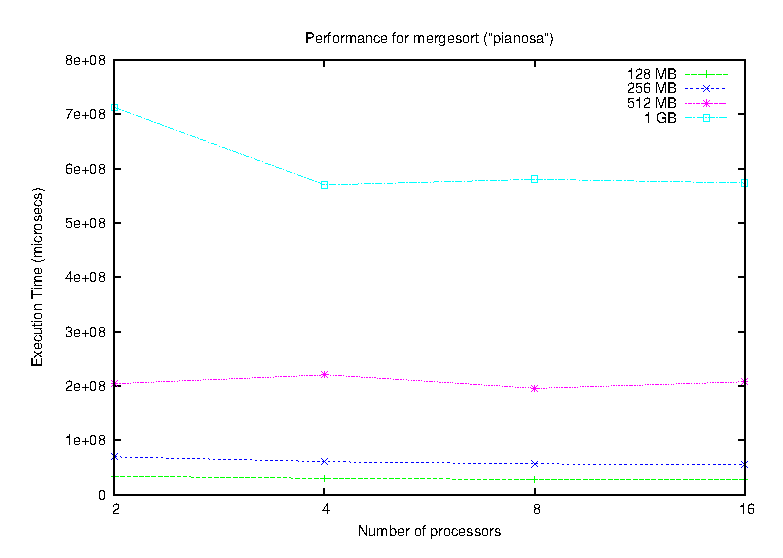
\includegraphics[width=0.4\textwidth]{plots/test_01_pianosa/NxTxM/mergesort_pianosa_NxTxM_large}}   
    \hspace*{20pt}  
    \subfloat[4-Way Mergesort.]{\label{NxTxM_large-kmerge}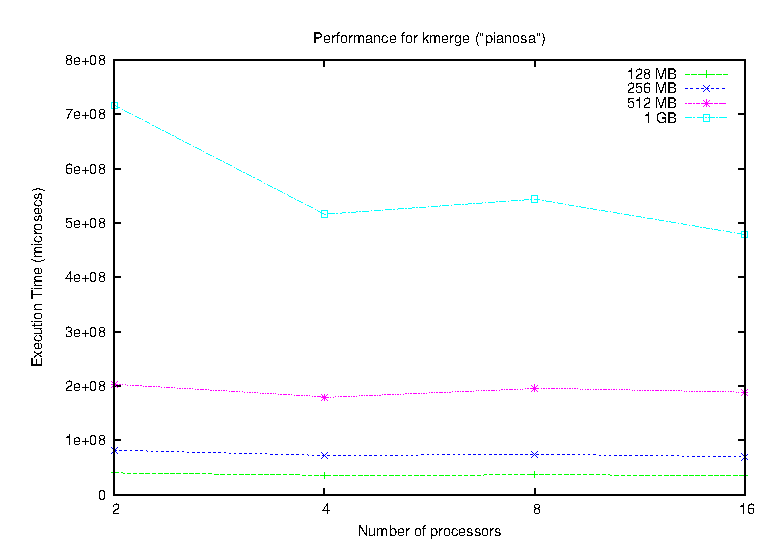
\includegraphics[width=0.4\textwidth]{plots/test_01_pianosa/NxTxM/kmerge_pianosa_NxTxM_large}} 
    
    \centering
    \subfloat[Load-Balanced Mergesort.]{\label{NxTxM_large-lbmergesort}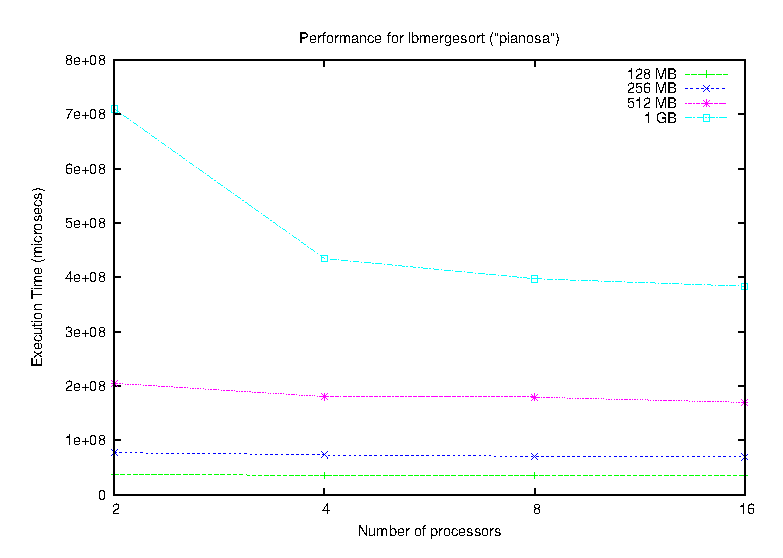
\includegraphics[width=0.4\textwidth]{plots/test_01_pianosa/NxTxM/lbmergesort_pianosa_NxTxM_large}} 
    \hspace*{20pt}  
    \subfloat[Load-Balanced Multi-Way Mergesort.]{\label{NxTxM_large-lbkmergesort}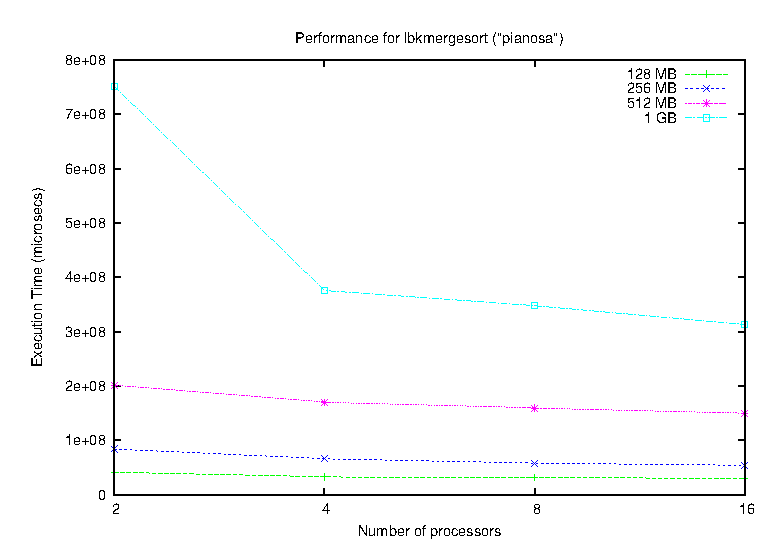
\includegraphics[width=0.4\textwidth]{plots/test_01_pianosa/NxTxM/lbkmergesort_pianosa_NxTxM_large}}  
    
\end{figure}
  



%%%%%%%%%%%%%%%%%%%%%%%%%%%%%%%%%%%%%%%% Huge data set %%%%%%%%%%%%%%%%%%%%%%%%%%%%%%%%%%%%%%%%%%%%%%%%%%%%%%
\begin{figure}[h]
	\ContinuedFloat
	
    \centering
    \subfloat[Quicksort.]{\label{NxTxM_huge-quicksort}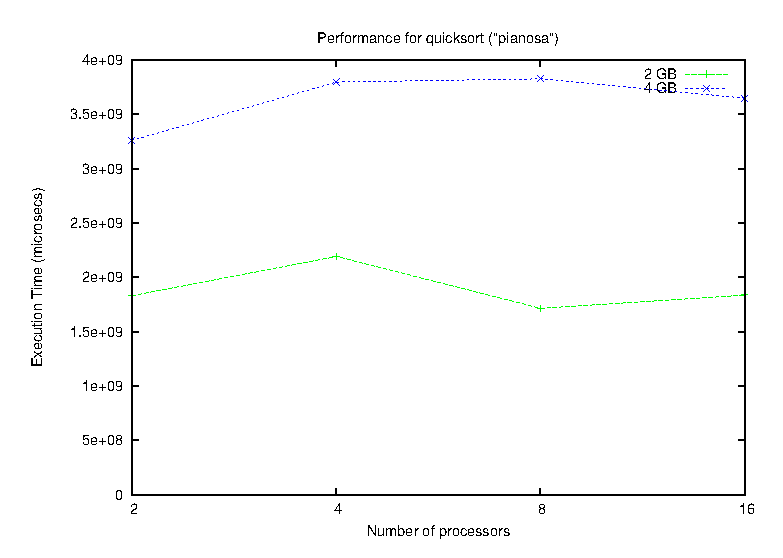
\includegraphics[width=0.4\textwidth]{plots/test_01_pianosa/NxTxM/quicksort_pianosa_NxTxM_huge}} 
    \hspace*{20pt}  
    \subfloat[Bitonicsort.]{\label{NxTxM_huge-bitonicsort}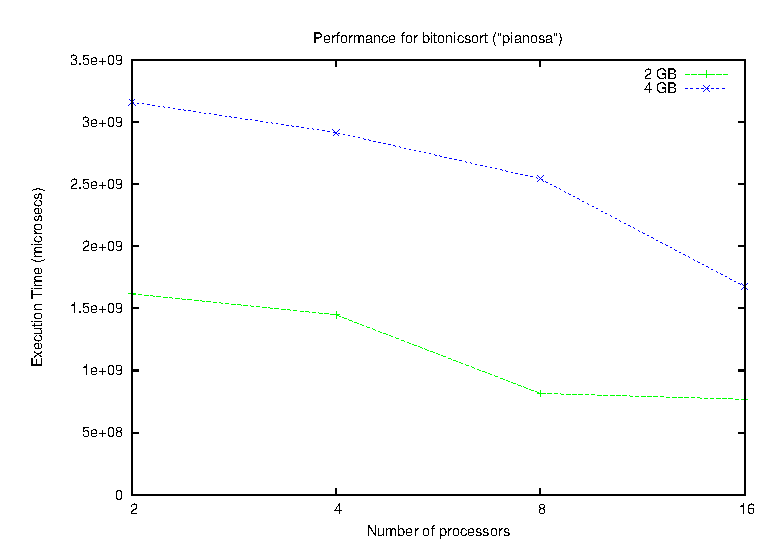
\includegraphics[width=0.4\textwidth]{plots/test_01_pianosa/NxTxM/bitonicsort_pianosa_NxTxM_huge}} 
    
    \centering
    \subfloat[Bucketsort.]{\label{NxTxM_huge-bucketsort}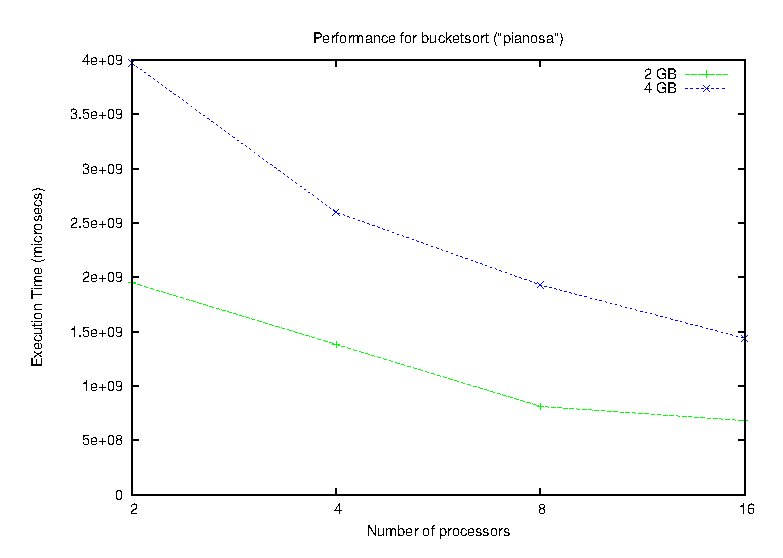
\includegraphics[width=0.4\textwidth]{plots/test_01_pianosa/NxTxM/bucketsort_pianosa_NxTxM_huge}} 
    \hspace*{20pt}
    \subfloat[Samplesort.]{\label{NxTxM_huge-samplesort}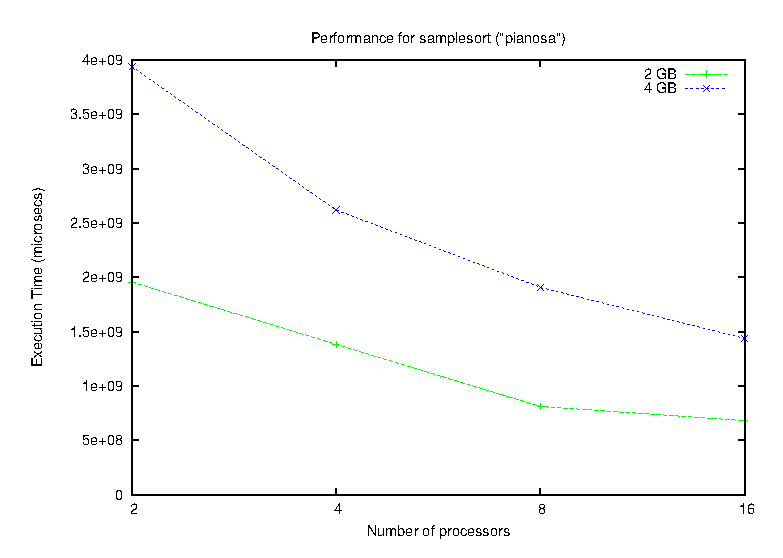
\includegraphics[width=0.4\textwidth]{plots/test_01_pianosa/NxTxM/samplesort_pianosa_NxTxM_huge}} 
    
    \centering
    \subfloat[Mergesort.]{\label{NxTxM_huge-mergesort}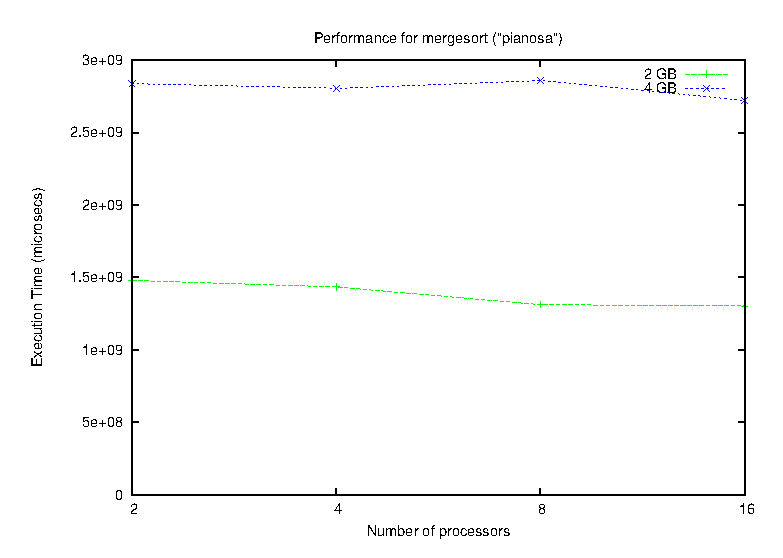
\includegraphics[width=0.4\textwidth]{plots/test_01_pianosa/NxTxM/mergesort_pianosa_NxTxM_huge}}   
    \hspace*{20pt}  
    \subfloat[4-Way Mergesort.]{\label{NxTxM_huge-kmerge}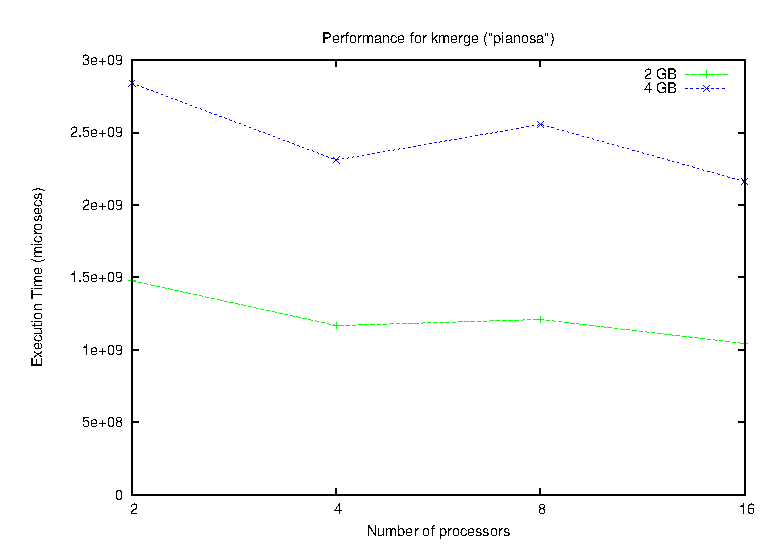
\includegraphics[width=0.4\textwidth]{plots/test_01_pianosa/NxTxM/kmerge_pianosa_NxTxM_huge}} 
    
    \centering
    \subfloat[Load-Balanced Mergesort.]{\label{NxTxM_huge-lbmergesort}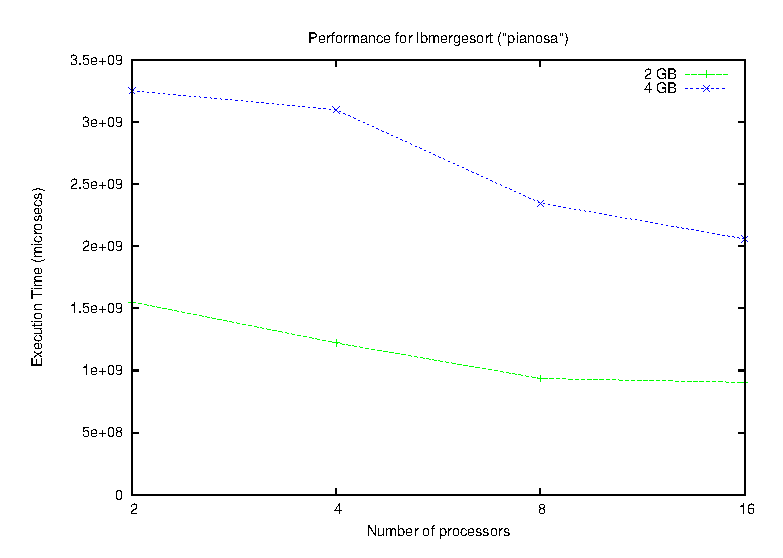
\includegraphics[width=0.4\textwidth]{plots/test_01_pianosa/NxTxM/lbmergesort_pianosa_NxTxM_huge}} 
    \hspace*{20pt}  
    \subfloat[Load-Balanced Multi-Way Mergesort.]{\label{NxTxM_huge-lbkmergesort}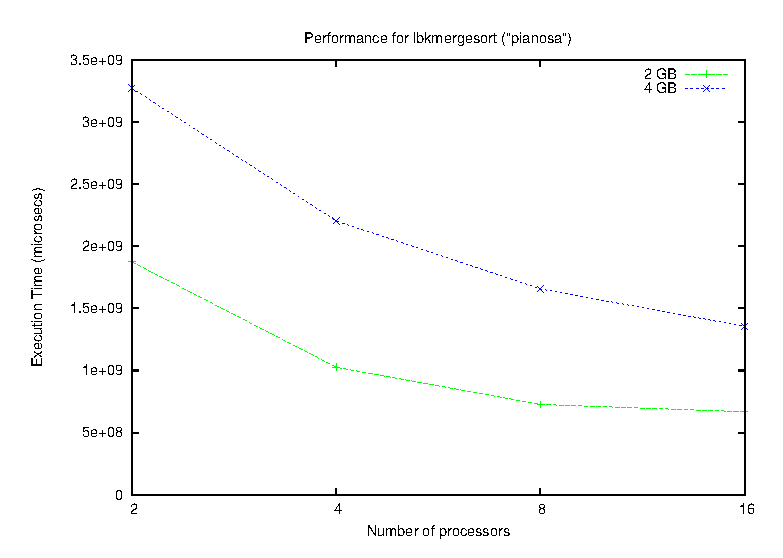
\includegraphics[width=0.4\textwidth]{plots/test_01_pianosa/NxTxM/lbkmergesort_pianosa_NxTxM_huge}}  
    
    \caption{\textit{Pianosa}. Time Completion of Sorting Algorithms by varying the parallelism degree. Each shape on a graphic represents the Time Completion of a certain Sorting Algorithm for a data set of specific size.}
    \label{NxTxM}
\end{figure}
  
 
\begin{figure}[!ht]
    \centering
    \subfloat[Quicksort.]{\label{MxTxN-quicksort}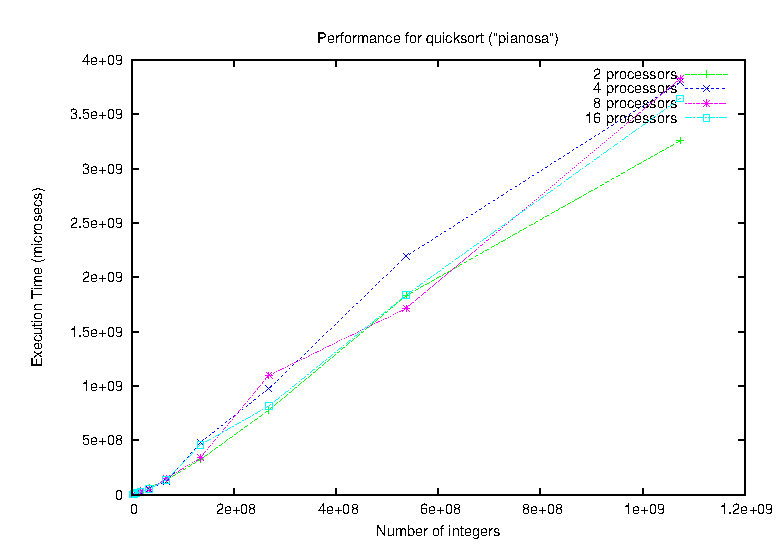
\includegraphics[width=0.4\textwidth]{plots/test_01_pianosa/MxTxN/quicksort_pianosa_MxTxN}} 
    \hspace*{20pt}  
    \subfloat[Bitonicsort.]{\label{MxTxN-bitonicsort}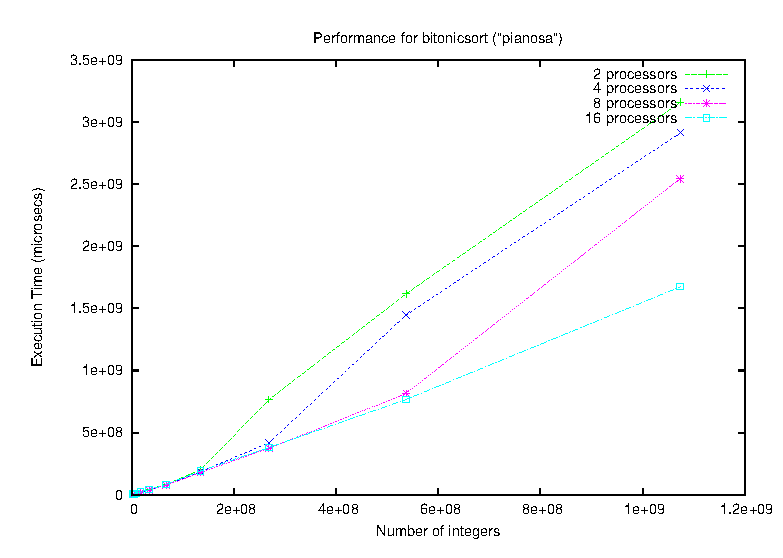
\includegraphics[width=0.4\textwidth]{plots/test_01_pianosa/MxTxN/bitonicsort_pianosa_MxTxN}} 
        
    \centering
    \subfloat[Bucketsort.]{\label{MxTxN-bucketsort}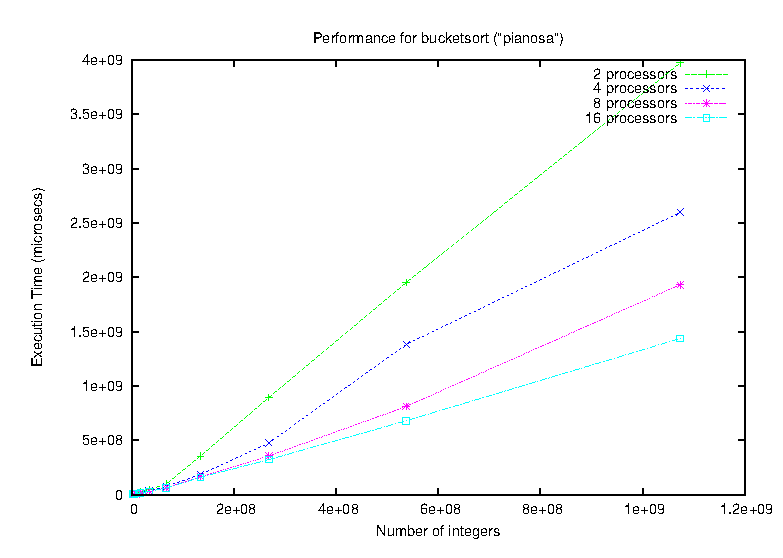
\includegraphics[width=0.4\textwidth]{plots/test_01_pianosa/MxTxN/bucketsort_pianosa_MxTxN}} 
    \hspace*{20pt}
    \subfloat[Samplesort.]{\label{MxTxN-samplesort}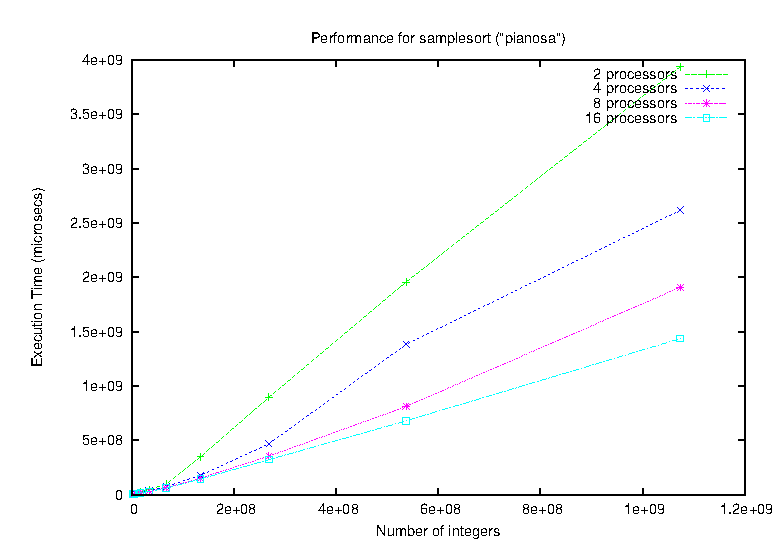
\includegraphics[width=0.4\textwidth]{plots/test_01_pianosa/MxTxN/samplesort_pianosa_MxTxN}} 
    
    \centering
    \subfloat[Mergesort.]{\label{MxTxN-mergesort}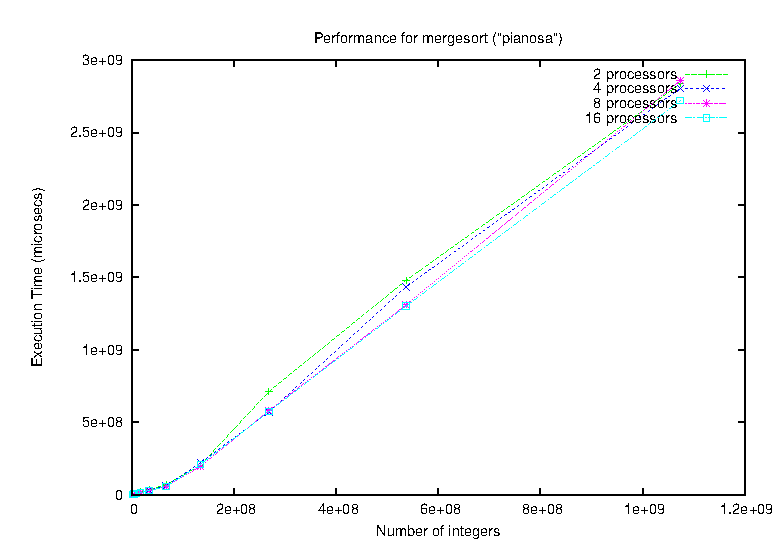
\includegraphics[width=0.4\textwidth]{plots/test_01_pianosa/MxTxN/mergesort_pianosa_MxTxN}}   
    \hspace*{20pt}  
    \subfloat[4-Way Mergesort.]{\label{MxTxN-kmerge}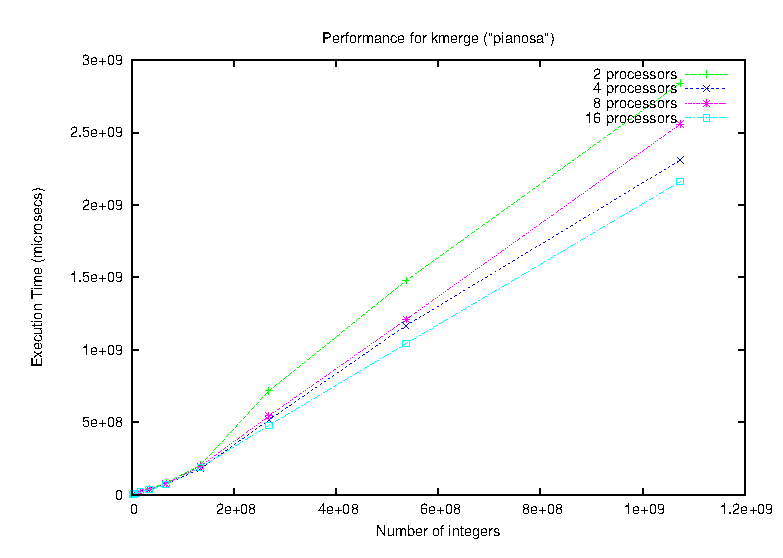
\includegraphics[width=0.4\textwidth]{plots/test_01_pianosa/MxTxN/kmerge_pianosa_MxTxN}} 
    
    \centering
    \subfloat[Load-Balanced Mergesort.]{\label{MxTxN-lbmergesort}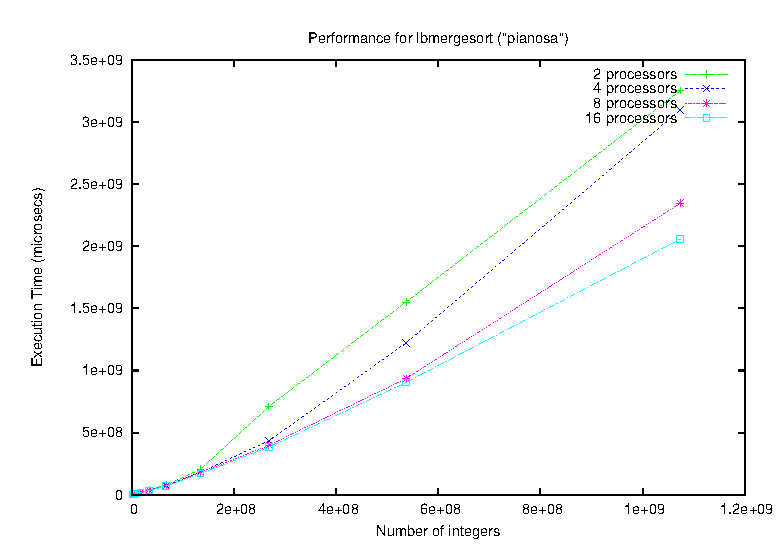
\includegraphics[width=0.4\textwidth]{plots/test_01_pianosa/MxTxN/lbmergesort_pianosa_MxTxN}} 
    \hspace*{20pt}  
    \subfloat[Load-Balanced Multi-Way Mergesort.]{\label{MxTxN-lbkmergesort}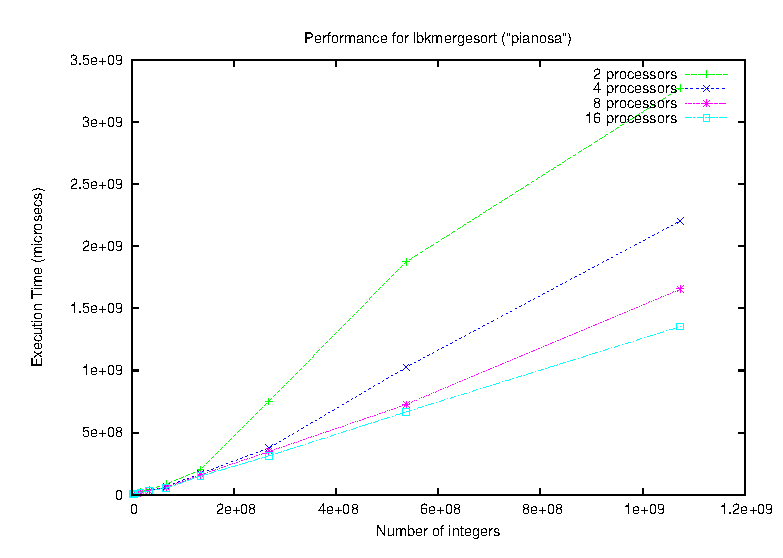
\includegraphics[width=0.4\textwidth]{plots/test_01_pianosa/MxTxN/lbkmergesort_pianosa_MxTxN}} 
    
    \caption{\textit{Pianosa}. Time Completion of Sorting Algorithms for increasing sizes of the data set. }
    \label{MxTxN}
\end{figure} 

\paragraph{Comparison between Sorting Algorithms}
In the previous section we have analyzed the scalability of singles Sorting Algorithms for different sizes of the data set. Now, we focus on determining the best Sorting Algorithm, in terms of Time Completion, for different sizes of the data set. First of all, recall that whether a data set fits the primary memory, a call to \textit{Sequentialsort} is simply a call to the standard \textit{ANSI qsort} (see chapter~\ref{sort-fram}). Therefore, in case of \textbf{small} data sets, the \textit{Sequentialsort} is the best algorithm we can use. Indeed, as we have already anticipated, in these cases the overhead of the parallelization is greater than the time that we would spend in a sequential, optimized computation, like the one of \textit{qsort}. On the other hand, things are obvioulsy different for larger data sets. Figures~\ref{NxTxA-large} and~\ref{NxTxA-huge} can be used to derive which algorithms exhibit the best Time Completions respectively for large and huge data sets. First, we consider the case of \textbf{large} data sets. 
Aside the \textit{Quicksort}, which suffers the unbalancing of the load among processes (see Appendix~\ref{appendix} for more details), most of the Sorting Algorithms outperform \textit{Sequentialsort}, at least when the size of the data set is greater than 4M integers. At least up to parallelism degree 16, the best algorithm is \textit{Mergesort}: in the best case, it is able to lower the Time Completion of \textit{qsort} of roughly 25$\%$ (see Figure~\ref{NxTxA-32M}). Now, we move to \textit{huge} data sets. It has been a great pleasure to see that the \textit{Load-Balanced Multi-Way Mergesort} (the Sorting Algorithm we designed and implemented by taking cue from \textit{Load-Balanced Mergesort}) is the algorithm that shows \textit{always} the best Time Completion (see also Figures~\ref{MxTxA-n4},~\ref{MxTxA-n8} and~\ref{MxTxA-n16}). Unfortunately, the lack of further machines to increase the parallelism degree at least up to 32 prevents the possibility of claiming deeper conclusions on these aspects. 


\begin{figure}[!ht]
	\centering
	\subfloat[Data set of 1M integers.]{\label{NxTxA-1M}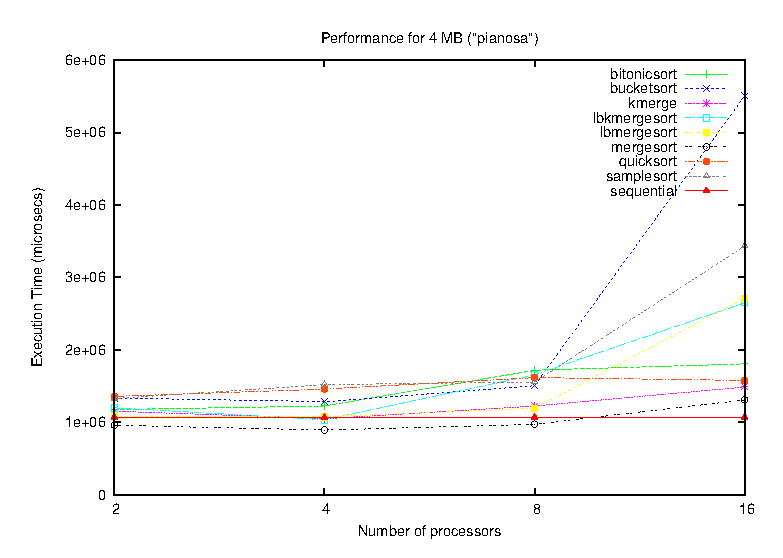
\includegraphics[width=0.4\textwidth]{plots/test_01_pianosa/NxTxA/M1048576_pianosa_NxTxA}} 
	\hspace*{20pt}	
  	\subfloat[Data set of 2M integers.]{\label{NxTxA-2M}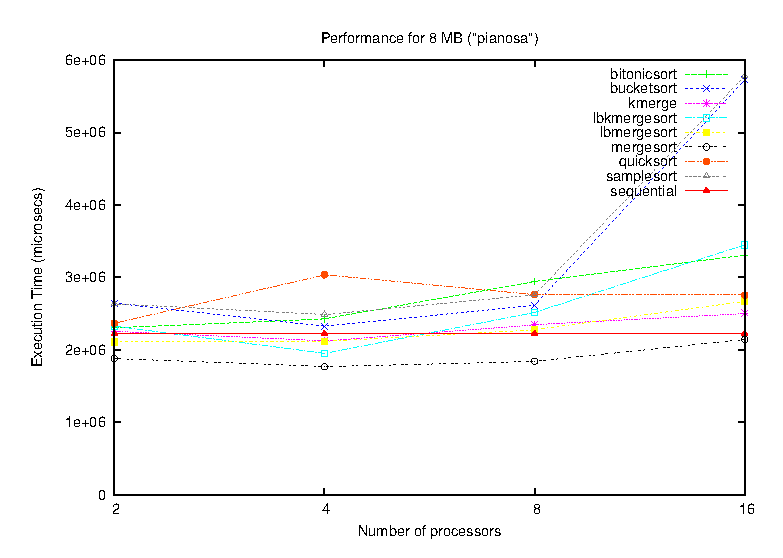
\includegraphics[width=0.4\textwidth]{plots/test_01_pianosa/NxTxA/M2097152_pianosa_NxTxA}} 
  		
	\centering
	\subfloat[Data set of 4M integers.]{\label{NxTxA-4M}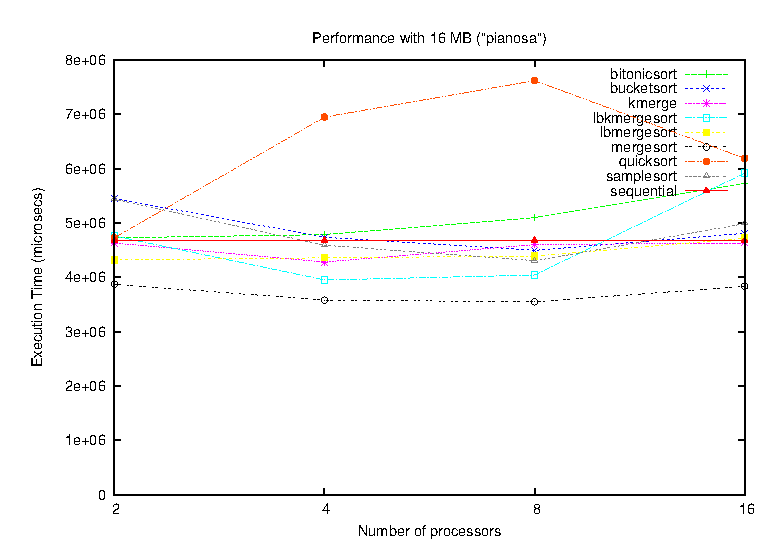
\includegraphics[width=0.4\textwidth]{plots/test_01_pianosa/NxTxA/M4194304_pianosa_NxTxA}} 
  	\hspace*{20pt}
  	\subfloat[Data set of 8M integers.]{\label{NxTxA-8M}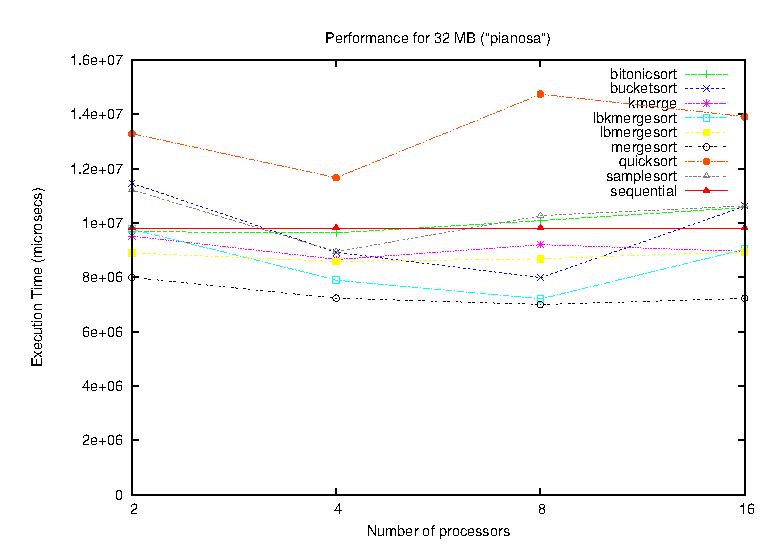
\includegraphics[width=0.4\textwidth]{plots/test_01_pianosa/NxTxA/M8388608_pianosa_NxTxA}} 
	
	\centering
  	\subfloat[Data set of 16M integers.]{\label{NxTxA-16M}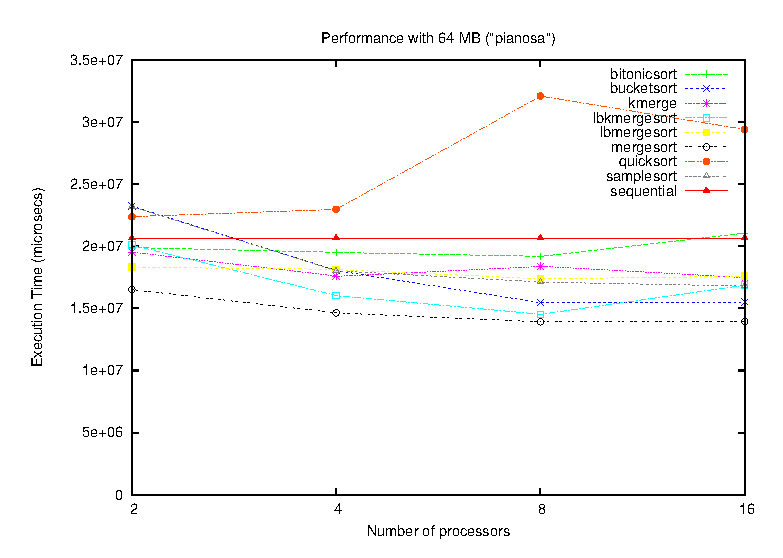
\includegraphics[width=0.4\textwidth]{plots/test_01_pianosa/NxTxA/M16777216_pianosa_NxTxA}}   
  	\hspace*{20pt}  
  	\subfloat[Data set of 32M integers.]{\label{NxTxA-32M}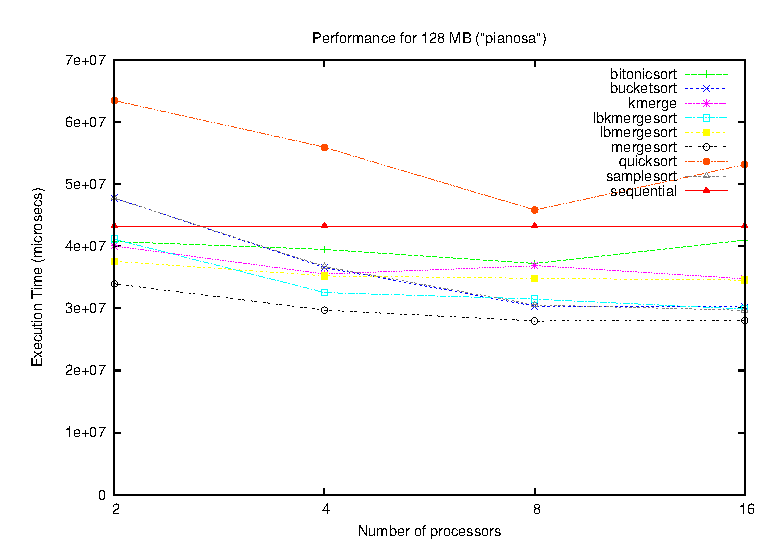
\includegraphics[width=0.4\textwidth]{plots/test_01_pianosa/NxTxA/M33554432_pianosa_NxTxA}} 
  	
	\caption{\textit{Pianosa}. Time Completion for sorting \textit{small} data sets. Each graphic represents a data set of fixed size, while each shape on a graphic shows the Time Completion of a certain Sorting Algorithm for that data set.}
	\label{NxTxA-small}
\end{figure} 

\begin{figure}[!ht]
	\centering
	\subfloat[Data set of 64M integers.]{\label{Pianosa-NxTxA-64M}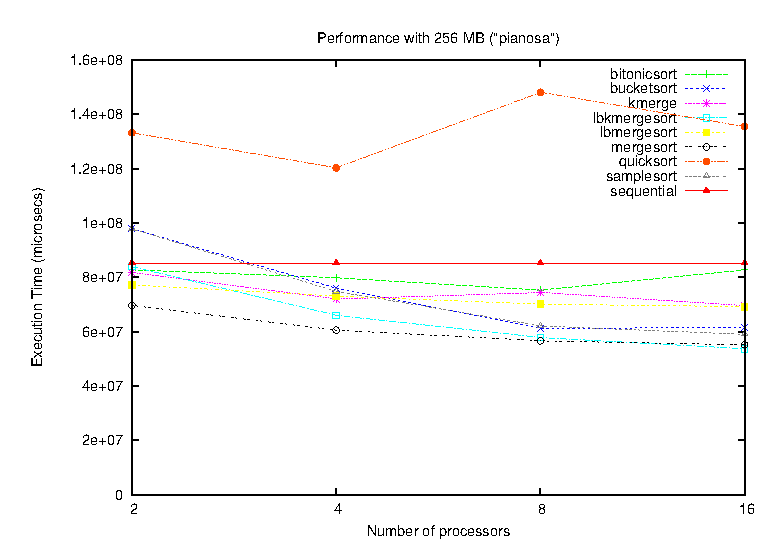
\includegraphics[width=0.5\textwidth]{plots/test_01_pianosa/NxTxA/M67108864_pianosa_NxTxA}} 
	
	\centering
  	\subfloat[Data set of 128M integers.]{\label{NxTxA-128M}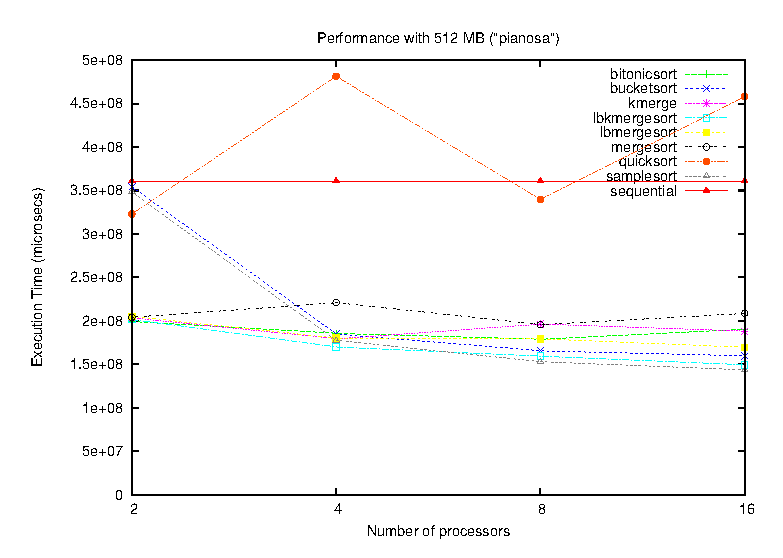
\includegraphics[width=0.5\textwidth]{plots/test_01_pianosa/NxTxA/M134217728_pianosa_NxTxA}} 
  		
	\centering
	\subfloat[Data set of 256M integers.]{\label{NxTxA-256M}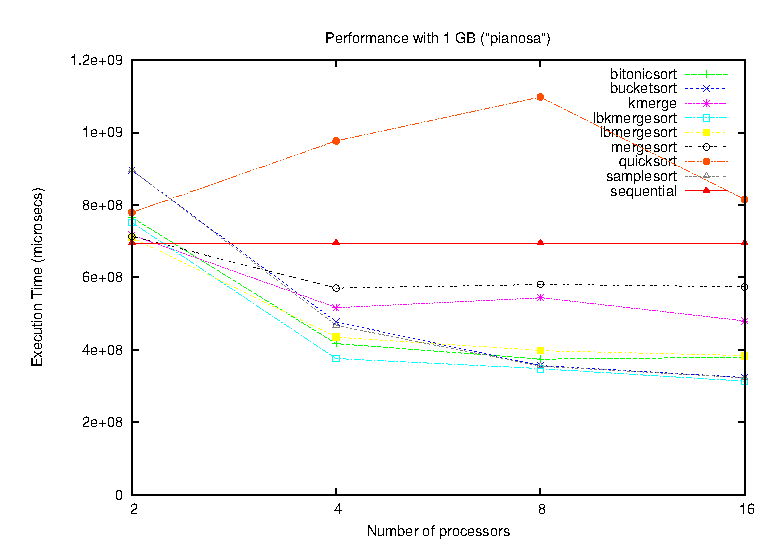
\includegraphics[width=0.5\textwidth]{plots/test_01_pianosa/NxTxA/M268435456_pianosa_NxTxA}} 
  	
  	\caption{\textit{Pianosa}. Time Completion for sorting \textit{large} data sets. Each graphic represents a data set of fixed size, while each shape on a graphic shows the Time Completion of a certain Sorting Algorithm for that data set.}
	\label{NxTxA-large}
\end{figure}

\begin{figure}[!ht]  	
  	\centering
  	\subfloat[Data set of 512M integers.]{\label{NxTxA-512M}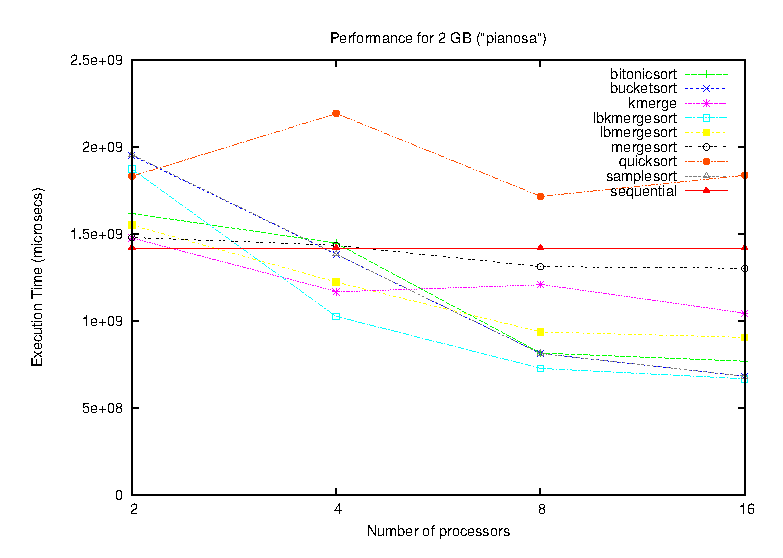
\includegraphics[width=0.6\textwidth]{plots/test_01_pianosa/NxTxA/M536870912_pianosa_NxTxA}} 
	
	\centering
  	\subfloat[Data set of 1G integers.]{\label{NxTxA-1G}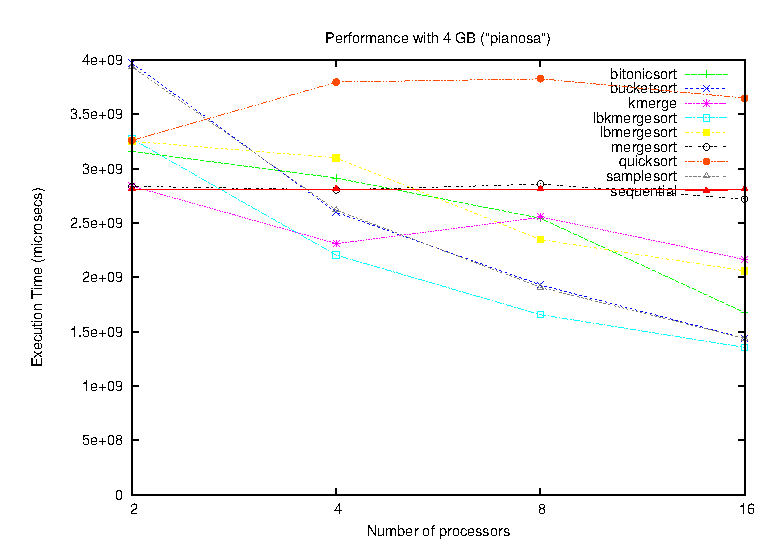
\includegraphics[width=0.6\textwidth]{plots/test_01_pianosa/NxTxA/M1073741824_pianosa_NxTxA}}    
  	
	\caption{\textit{Pianosa}. Time Completion for sorting \textit{huge} data sets. Each graphic represents a data set of fixed size, while each shape on a graphic shows the Time Completion of a certain Sorting Algorithm for that data set.}
	\label{NxTxA-huge}
\end{figure} 

\begin{figure}[!ht]
	\centering
	\subfloat[Parallelism degree 2.]{\label{MxTxA-n2}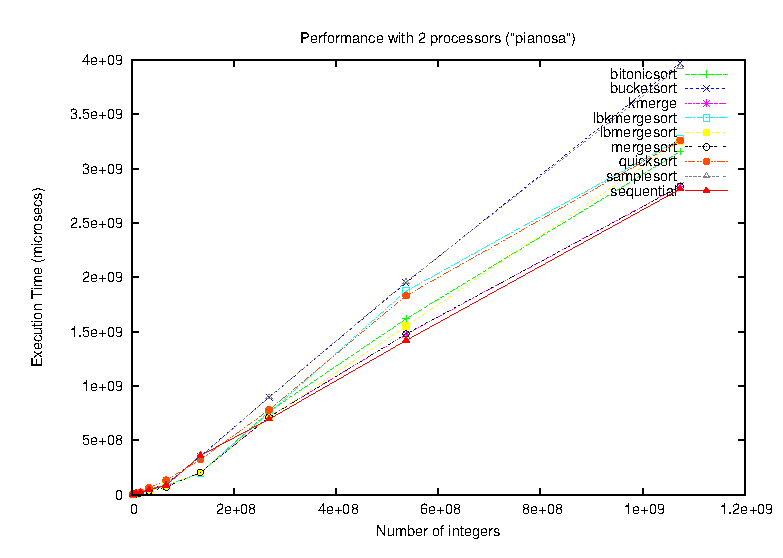
\includegraphics[width=0.4\textwidth]{plots/test_01_pianosa/MxTxA/n2_pianosa_MxTxA}} 
	\hspace*{20pt}	
  	\subfloat[Parallelism degree 4.]{\label{MxTxA-n4}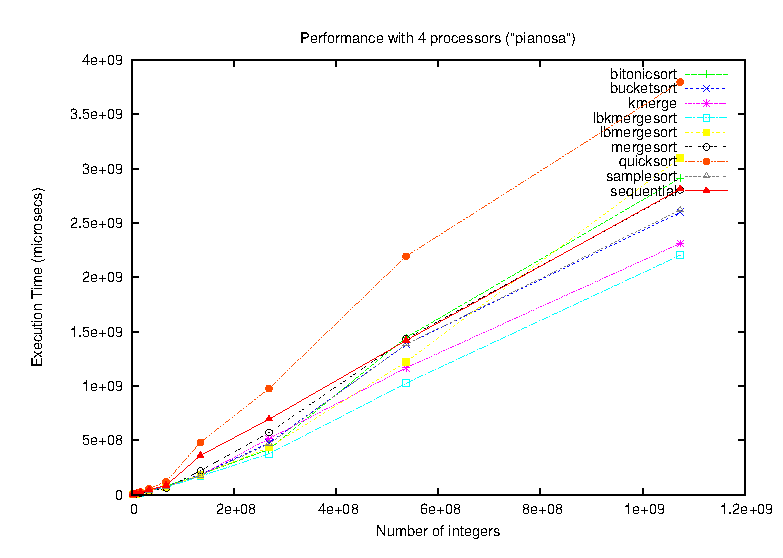
\includegraphics[width=0.4\textwidth]{plots/test_01_pianosa/MxTxA/n4_pianosa_MxTxA}} 
  		
	\centering
	\subfloat[Parallelism degree 8.]{\label{MxTxA-n8}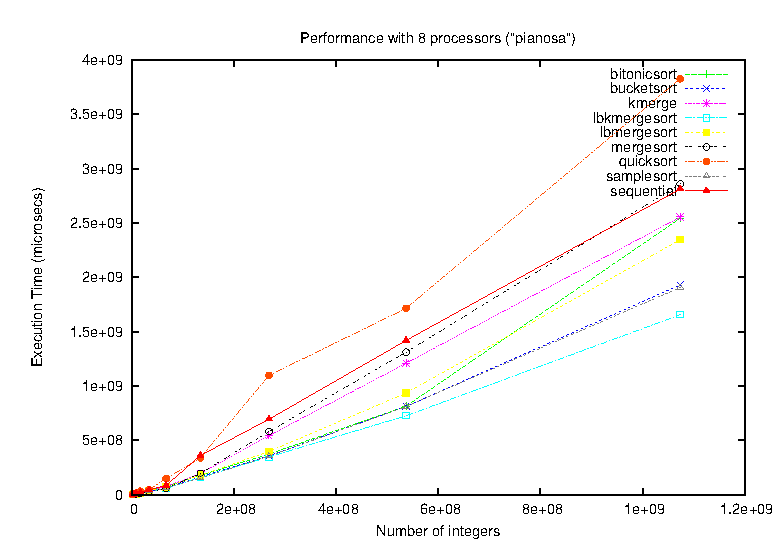
\includegraphics[width=0.4\textwidth]{plots/test_01_pianosa/MxTxA/n8_pianosa_MxTxA}} 
  	\hspace*{20pt}
  	\subfloat[Parallelism degree 16.]{\label{MxTxA-n16}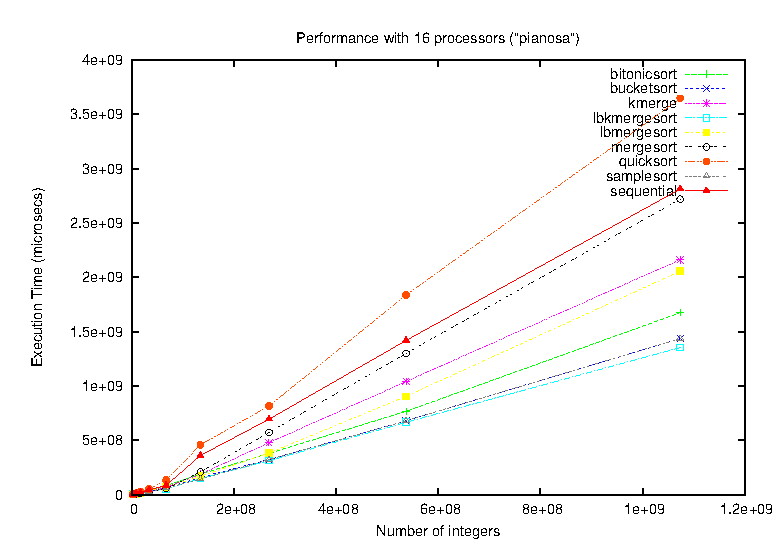
\includegraphics[width=0.4\textwidth]{plots/test_01_pianosa/MxTxA/n16_pianosa_MxTxA}} 
  	
	\caption{\textit{Pianosa}. Time Completion for sorting data sets with fixed parallelism degree.}
	\label{MxTxA}
\end{figure} 

\clearpage